\documentclass[usenatbib,fleqn]{mnras}

\makeatletter
\newlength{\abovecaptionskip}%
\setlength{\abovecaptionskip}{10\p@}
\makeatother


\usepackage{threeparttable}
 

\usepackage{amsmath,amssymb}
\usepackage{mathrsfs}
\usepackage{graphicx}
\usepackage{epstopdf}
%\usepackage{hyperref}
\epstopdfsetup{outdir=./figures/}
\graphicspath{{./figures/}}
\usepackage{url}
%\usepackage{aas_macros}

\newcommand\lsim{\mathrel{\rlap{\lower4pt\hbox{\hskip1pt$\sim$}}
    \raise1pt\hbox{$<$}}}
\newcommand\gsim{\mathrel{\rlap{\lower4pt\hbox{\hskip1pt$\sim$}}
    \raise1pt\hbox{$>$}}}

\newcommand{\Mbh}[1][]{M_{\bullet#1}}
\newcommand{\Menc}{M_{\rm enc}}
\renewcommand{\th}{t_h}
\newcommand{\Msun}{{\rm M_\odot}}
\newcommand{\pyear}{{\rm yr}^{-1}}

% write title (with email and institute)
\title{TDE jets}

\begin{document}

\begin{abstract}
  Radio light curves calculated for TDE jets. CNM
  densities based on \citet{Generozov+2015}. 
\end{abstract}
\section{Introduction}
\label{sec:intro}
When a star in a galactic nucleus is deflected too close to the central supermassive black hole (BH), it can be torn apart by tidal forces.  During this tidal disruption event (TDE), roughly half of the stellar debris remains bound to the BH, while the other half is flung outwards and unbound from the system.  The bound material, following a potentially complex process of debris circularization (\citealt{Guillochon&RamirezRuiz13},\citealt{Hayasaki+15}), accretes onto the BH, creating a luminous flare lasting months to years \citep{Hills1975, Carter+1982, Rees1988}. 

Many thermal TDE flares have now been identified at UV/optical \citep{van-Velzen+2011, Gezari+2012, Chornock+2014,
  Arcavi+2014} and/or soft x-ray wavelengths \citep{Esquej+2007}.  Beginning with the discovery of {\it Swift} J1644+57 in 2011,
three additional TDEs have been discovered by their non-thermal non-thermal x-ray emission (\citealt{Bloom+2011, Levan+2011, Burrows+2011, Zauderer+2011, Cenko+2012, Pasham+2015, Brown+2015}), which is believed to be the result of emission from a relativistic jet beamed along our line of sight.   In addition to their highly variable X-ray emission, which likely originates from the base of the jet, these events are characterized by radio synchrotron emission.  The latter, more slowly evolving, is powered by shocks formed at the interface between the jet and surrounding circumnuclear medium (CNM) (\citealt{Giannios&Metzger11,Metzger+12}), analagous to the afterglow of a gamma-ray burst.

Although a handful of such jetted TDE flares are now known, their observed volumetric rate is a very small fraction $\sim 10^{-4}$ of the rate of observed thermal TDE flares (e.g., \citealt{Burrows+11}), and an even smaller fraction of the theoretically predicted TDE rate (\citealt{Stone&Metzger14}).  One explanation for this discrepency is that the majority of TDEs indeed produce jets, but the their non-thermal X-ray emission is relativistically beamed into a very small angle $\theta_{\rm b}$.  However, in order to explain the required beaming fraction $f_b \approx \theta_{b}^{2}/2 \sim 10^{-4}$ would require $\theta_{\rm b} \sim 0.01$ and hence a jet with a bulk Lorentz factor of $\Gamma \gtrsim 1/\theta_j \sim 100$, much higher than typically inferred for AGN jets or inferred for {\it Swift} J1644+57 (\citealt{Metzger+12}).  

The detection rate of non-thermal TDE may instead indicate that jets are intrinsically rare in TDEs, or the conditions in the surrounding environment are unfavorable for producing bright emission.  Jets could be rare if they require a highly super-Eddington accretion (\citealt{DeColle+12}), a deeply plunging TDE (\citealt{Metzger&Stone15}), or a particularly strong magnetic flux threading the star (\citealt{Tchekhovskoy+14,Kelley+15}).  Alternatively, jet formation or X-ray emission could be hampered by Lens-Thirring precession of the accretion disk caused by the misalignment between the angular momentum of the BH and that of the disrupted star (\citealt{Stone&Loeb12}).  In the latter case, even a `messy' jet could still produce non-thermal radio synchrotron emission as it shocks and interacts with the surrounding CNM, and this emission is predicted to be relatively isotropic (\citealt{Metzger&Giannios11},\citealt{Mimica+15}).  

Observational campaigns have been conducted to follow-up thermal TDE flares at radio wavelengths on timescales of months to decades after the outburst (\citealt{Bower+13}; \citealt{van-Velzen+2013}).  \citet{Bower+13} detected radio emission from the candidate TDE flares RX J1420.4+5334 and IC 3599.  However, for RX J1420.4+5334 the radio emission was observed in a different galaxy than that originally identified by \citet{Komossa&Greiner99} as the host.  The highly irregular behavior of IC 3599 (e.g.~\citealt{Campana+15}) has also called into question whether this event is a true TDE at all.  In all other cases, observations have resulted in only upper limits.  Based on simple models for the radio emission from the Sedov blastwave, \citet{Bower+13} and \citet{van-Velzen+2013} conclude that $\lesssim 10\%$ of TDEs produce jetted TDE emission similar to {\it Swift} J1644+57.


  There are two general classes of explanation for this discrepency (1) jets are launched in the majority of TDEs, but
the typical CNM density is unfavorable for producing observable synchrotron emission. (2) Powerful relativistic jets are intrinsically
uncommon in tidal disruption events.

In this paper we check whether the first possibility by simulating the
jet-CNM interaction across the range of physically expected
circumnuclear medium densities.  We fix the jet properties to the best
jet model from \citet{Mimica+2015} for the Sw J1644+57 tidal
disruption flare. If it turns out that such a jet would produce
observable radio emission for all physical circumnuclear densities,
then it must that most tidal disruption events do not launch
J1644-like jets.  Speculatively, this could be because stars typically
do not carry sufficient magnetic flux for the Blandford-Znajek
mechanism {\bf AG: cite!} to operate. In any case, this would have
significant implications for jet launching physics.

% We simulate the hydrodynamic interaction of the jet with the CNM in
% one and two-dimensions, and calculate resulting synchrotron emission,
% as done by \citet{Mimica+2015}.  This is a two component jet with a fast
% ($\Gamma=10$) core and a slow ($\Gamma=2$) sheath with isotropic
% equivalent energy $E=4 \times 10^{54}$ ergs {\bf AG--Modification for
%   reproducing 2-d sims...}.
{\bf AG I commented out a paragraph here describing some of the
  details of the jet model, but I think this could actually go in a
  different section.}

To establish low and high density limits for the circumnuclear gas, we
consider the rate of mass injection from stellar winds for different
stellar populations. A younger stellar population would have
significant wind mass loss from O \& B stars. In contrast, these rate
of wind mass loss from an older population, which lacks these massive
stars, could $\sim 2$ orders of magnitude smaller. We use the
formalism of \citet{Generozov+2015} (hereafter GSM15) to estimate CNM
gas density for a broad range of stellar populations. By comparing the
radio light-curves with observed radio upper limits, we test whether
TDE jets would produce observable synchrotron emission for the
physically expected range of CNM densities.

The remainder of the this paper is organized as follows: In
$\S\ref{sec:cnm}$ we bracket the range of physically expected CNM
densities. In $\S\ref{sec:jet}$ we describe the our model for the TDE
jet and the jet-CNM interaction. We use both 1d and 2d hydrodynamic
models to simulate the jet propagating through the CNM and compare the
results in $\S\ref{sec:2d}$. In $\S\ref{sec:results}$ we show radio
light-curves from our 1d models for a wide range of CNM densities, to
illustrate qualitatively how much varying the CNM density by itself
could change the radio light-curve.  We discuss the implications of
our models for detections of TDEs by future radio surveys in
$\S\ref{sec:disc}$, and summarize our conclusions in
$\S\ref{sec:conc}$.

\section{CNM density}
\label{sec:cnm}

\subsection{Model}

The density profile of the CNM encountered by a relativistic TDE jet
will affect the observed radio light curve. A very high density could
rapidly decelerate the jet, suppressing the synchrotron emission.
{\bf AG more details.}  It could be radio emission from TDE jets is
only observable for a narrow range of CNM properties. Although the
empirical rate of jetted tidal disruption events is small (0.1-10\% of
the TDE rate according to \citealt{van-Velzen+2013}) it is possible
that the intrinsic rate is far higher.

We calculate radio light curves for a range of physically plausible
CNM densities, to explore what conditions are required for TDE jets to
produce observable radio emission. 

The dominant source of gas injection into the CNM of quiescent
galaxies is winds from stars in the galactic nucleus. The 1D spherical
hydrodynamic equations with stellar wind mass injection are
(e.g. \citealt{Holzer+1970}) {\bf AG: possibly the detailed
  description of the CNM model should get a separate appendix.}


\begin{align}
  &\frac{\partial \rho}{\partial t}+\frac{1}{r^2}\frac{\partial}{\partial r}\left(\rho r^2 v\right)=q \label{eq:drhodt}\\
  &\rho \left(\frac{\partial v}{\partial t} + v\frac{\partial
      v}{\partial r}\right) =-\frac{\partial p}{\partial r}- \rho\frac{GM_{\rm enc}}{r^{2}} -q v \label{eq:dvdt}\\
  &\rho T\left(\frac{\partial s}{\partial t} + v\frac{\partial
      s}{\partial
      r}\right)=q\left[\frac{v^2}{2}+\frac{v_w^2}{2}-\frac{\gamma}{\gamma-1}
    \frac{p}{\rho} \right] ,
\label{eq:dsdt}
\end{align}

where $\rho$, $v$, $p$, and $s$ are the density, velocity, pressure, and
specific entropy, respectively.  $\Menc$ is the combined black hole
and enclosed stellar mass. The pressure is given by an ideal gas
equation of state.  {\bf AG: Quick summary of previous work on
  modeling CNM density.}

 {\bf AG: note I took the mean molecular weight to be
  0.62.}

$q$ is the mass injection rate per unit volume per unit time and is
proportional the stellar density divided by a Hubble time: $q=\eta
\rho_\star/\th$. $v_w$ encapsulates the heating of the gas. Physically
this may come from (1) the stellar wind kinetic energy (2) supernovae
(3) black hole feedback.

\citet{Generozov+2015} find that the gas density depends on the
mass return parameter, $\eta$, the heating rate, $v_w$, the black hole
mass, $\Mbh$, and the power law slope of the stellar density profile
($\rho_\star\sim r^{-\delta_1}$ for small radii).

For a cusp galaxy ($\delta_1> 0.5$), the gas density, $\rho\sim
r^{-1}$. In this case the gas density at $10^{18}$ cm, $n_{18}$ can be
approximated using a simple scaling relation 

\begin{equation}
n_{18}\simeq 0.4 \Mbh[,7]^{0.5} \eta_{0.02} v_{500}^{-1.5} {\rm
  cm^{-3}},
\label{eq:n18}
\end{equation}

where $\Mbh[,7]=\frac{\Mbh}{10^7 \Msun}$,
$\eta_{0.02}=\frac{\eta}{0.02}$, and $v_{500}=\frac{v_w}{500 {\rm
    km/s}}$, and we have assumed a fixed slope for the stellar density
power law slope $\delta_1=1.8$. Thus, the gas density is quite
sensitive to the mass return parameter and the heating rate, which are
related to the star formation history. Young, massive stars put out
very energetic winds with $v_w\simeq 1000$ km/s with a high mass
return rate, $\eta\simeq 100$, in contrast stars with age comparable
to that of the universe will have slow winds with speeds of order $\sim
10$ km/s and mass return parameters, $\eta\simeq0.02$. In the next
section we explore the range of mass return parameters, heating rates,
and gas densities allowed by plausible star formation histories.

\subsection{Plausible range of CNM gas densities}
Increasing the mass return parameter, $\eta$, or decreasing the
heating parameter $v_w$, increases the gas density, $n_{18}$.
However, one cannot increase the $\eta$ or decrease $v_w$ arbitrarily
as the CNM will become thermally unstable. Specifically if the heating
rate falls below

\begin{equation}
v_{\rm w,TI}\simeq 200 \eta_{0.02}^{0.17} \Mbh[,7]^{0.08} \,{\rm km/s} 
\label{eq:ti}
\end{equation}

{\bf AG: for vw$>1000$ km/s the cooling will be dominated by
  Bremstrahlung and so the ti criterion may be somewhat different} {\bf
  AG: Note that properly interpreted this critical heating rate
  corresponds to the total heating--including the velocity dispersion
  heaitng.}  
If the heating rate falls below this critical value the
CNM will become thermally unstable, condensing into cold clouds {\bf
  AG--caveats}. Thus, the maximum possible density $n_{18}$ for a
given $\eta$ will correspond to $v_{\rm w,TI}$. From
equations~\eqref{eq:n18} and~\eqref{eq:ti} this will be given by

\begin{equation}
n_{\rm 18,TI}\simeq 1.6 \eta_{0.02}^{0.75} \Mbh[,7]^{0.38} \, {\rm cm^{-3}}
\label{eq:n18ti}
\end{equation}

The maximum physical $\eta\simeq 400$\footnote{For details
  of how to calculate $\eta$ for a given star formation history see
  appendix C of \citet{Generozov+2015}.} occurs $\sim 3$ Myr after a
burst of star formation. Evaluating equation~\eqref{eq:n18ti} with
$\eta=400$ gives the maximum possible CNM density

\begin{equation}
n_{\rm 18,max} \simeq 2,700 \Mbh[,7]^{0.38} {\rm cm^{-3}}
\label{eq:n18max}
\end{equation}

Although such large gas densities would be present in the immediate
aftermath of a starburst, the wind mass loss rate (and thus the gas
density) declines as $\eta \sim t^{-3}$. Thus we expect the gas density would
decline by an order of magnitude after a few Myr. Note that type II
Supernovae could inject additional mass into the CNM, but this
injection would be intermittent (e.g. the time between SNe would be
long compared to a dynamical time).

% {\bf AG the subsequent discussion relies on out of date parameters for
% the stellar light profile for NGC 3156. In calculating the profile, we
% assume it turns over at 2 pc. In reality it probably turns over at ~20
% pc, and becomes a typical cusp profile. Next few paragraphs should be axed.}
% However, we also find high gas densities ($n_{18}\sim 2000$ cm$^{-3}$)
% may be present for E+A galaxies with stellar ages $\tau_\star\sim
% 10^8-10^9$ years. Although E+A galaxies are rare they host $\sim 20
% \%$ of all optically selected TDE candidates. Thus, the high density
% limit could be relevant for a sizable fraction of TDEs {\bf AG citation
%   needed here...}

% {\bf AG too much detail?} We construct a gas density profile for the
% nearby E+A galaxy NGC 3156. This galaxy has a stellar light profile
% measured with high resolution HST photometry. \citealt{Krajnovic+2013}
% find a steep inner stellar density profile with $\rho_\star\sim
% r^{-2.78}$, albeit with a possible turnover to a shallower profile at
% $r \sim 2-4$ pc. We assume a core-like profile with $\rho_\star \sim
% r^{-1.1}$ for $r<2$ pc.

% We find a thermally stable profile for NGC 3156 for mass
% return parameter $\eta\simeq0.5$ and Type Ia supernova heating
% $v_w\simeq600 $ km/s, as expected for 1 Gyr after a burst of star
% formation. We find $n \sim 2000 (r/10^{18} {\rm cm})^{-1.3}$
% cm$^{-3}$, for $r<2$ pc, $n\sim r^{-2}$ for $r>2$ pc, which is quite
% similar to the profile for a normal cusp galaxy with break at $r_b$=2
% pc. {\bf AG--w/o turnover the inner density slope would be -2--possibly
% do a special case?}

% Such a large gas density should produce a large x-ray luminosity in
% the galactic nucleus from metal line cooling and free-free emission.
% In particular our model for the E+A galaxy predicts an x-ray
% luminosity of $\sim$ few $\times 10^{39}$ egs/s, from the inner few
% parsecs of the galaxy {\bf AG--reran with proper normalization of the
%   cooling function (this was incorrect in GSM15). Would be good to
%   double-check these results.}


% {\bf AG--we could probably look for archival ROSAT observations for
%   non-active galaxies, to constrain the gas densities
%   there. For any galaxy w/o central x-ray source could put upper
%   limits on the gas density based on the free-free emission we would
%   have to have.}
% We found an archival X-ray observation from ROSAT for this galaxy {\bf
%   AG describe observation here; look for other observation}. There are
% no X-ray sources consistent with the galactic nucleus, which gives a
% 90\% confidence of upper limit $<2.4$ counts over the $\sim$400 s
% exposure time. We then use this non-detection to put an upper limit on
% the unresolved x-ray flux from the galactic nucleus using the
% web-PIMMS
% tool\footnote{https://heasarc.gsfc.nasa.gov/cgi-bin/Tools/w3pimms/w3pimms.pl}. We
% use an APEC emission model, temperature of ($10^{7} K$--the
% approximate temperature of the gas for radii dominating the x-ray
% emission a solar metallicity ({\bf AG Check for metallicity
%   measurements for this galaxy}), and $2.43\times 10^{20} {\rm
%   cm^{-2}}$ for the galactic HI column density\footnote{from
%   https://heasarc.gsfc.nasa.gov/cgi-bin/Tools/w3nh/w3nh.pl}. With
% these parameters non-detection gives an upper limit on the flux of
% $\lsim 2\times 10^{39}$ ergs/s {\bf AG check for other x-ray
%   images}. Thus, the non-detection is marginally consistent with the
% model, though it shows the density cannot be much higher than we
% predict.

What is the smallest plausible CNM density? This would correspond to a
small mass return parameter and a high heating rate. The mass return
parameter, $\eta=0.02$, reaches its minimum value for a stellar
population that is a Hubble time old. A stellar population
that is $<$ 3 Myr old will have a heating rate, $v_w=3,000$ km/s.

A stellar population in which a small fraction, $f$ of the stars
formed $\lsim 3$ Myr ago and the rest are a Hubble time old, will have
both a high heating rate and a low mass return rate. In this scenario
$n_{18}$ will be minimized for $f=4\times 10^{-4}$. Both old and young
stars contribute significantly to the mass injection rate giving
$\eta\simeq 0.03$, while the young star dominate the heating
$v_w\simeq 3,000$ km/s and thermally stabilize the gas. These
parameters give us the minimum possible CNM gas density

\begin{equation}
n_{\rm 18,min}\simeq 0.06 \Mbh[,7]^{0.5} {\rm cm^{-3}}
\label{eq:n18min}
\end{equation}

We illustrate how the mass return parameter, heating rate, and
density vary with star formation history in Fig.~\ref{fig:param}. The
gray lines represent a two-burst model for star formation in which a
fraction, $f$, of the stars formed $<$ 3 Myr ago and the remainder
formed a Hubble time ago (top gray line) or 1 Gyr ago (bottom red
line).  Towards the top right the $f=1$ and the young stars dominate
the mass injection rate and the heating rate.  Moving towards the
left, $f$ decreases, along with the mass return rate, and density
(blue lines), but the heating rate, $v_w$, remains $\gsim 1000$ km/s
except for very small values of $f$. The bend in the top, solid, gray curve
corresponds to the minimum possible CNM density.

The dashed, gray line also represents a two burst formation history
but the older burst is $\sim 3$ Myr old (right at the age when stars
are beginning to leave the main sequence, increasing the mass
injection rate. Towards the lower right of the dashed, gray line these
somewhat older stars dominate the mass injection into the CNM,
increasing the density past the thermal instability threshold (thick,
black line). The intersection between the dashed gray line and the
thermal instability line corresponds to the maximum possible CNM
density.

{\bf AG--for these star formation histories there may be small numbers
of massive stars present. In particular for the low density limit we
would produce a stellar population, with 1 massive star within the
stagnation radius, in this case our formalism would break down.}

{\bf AG--Describe a more typical case of a 1 Gyr age stellar
  population, and heating coming from Ia supernova.}

\begin{figure} 
  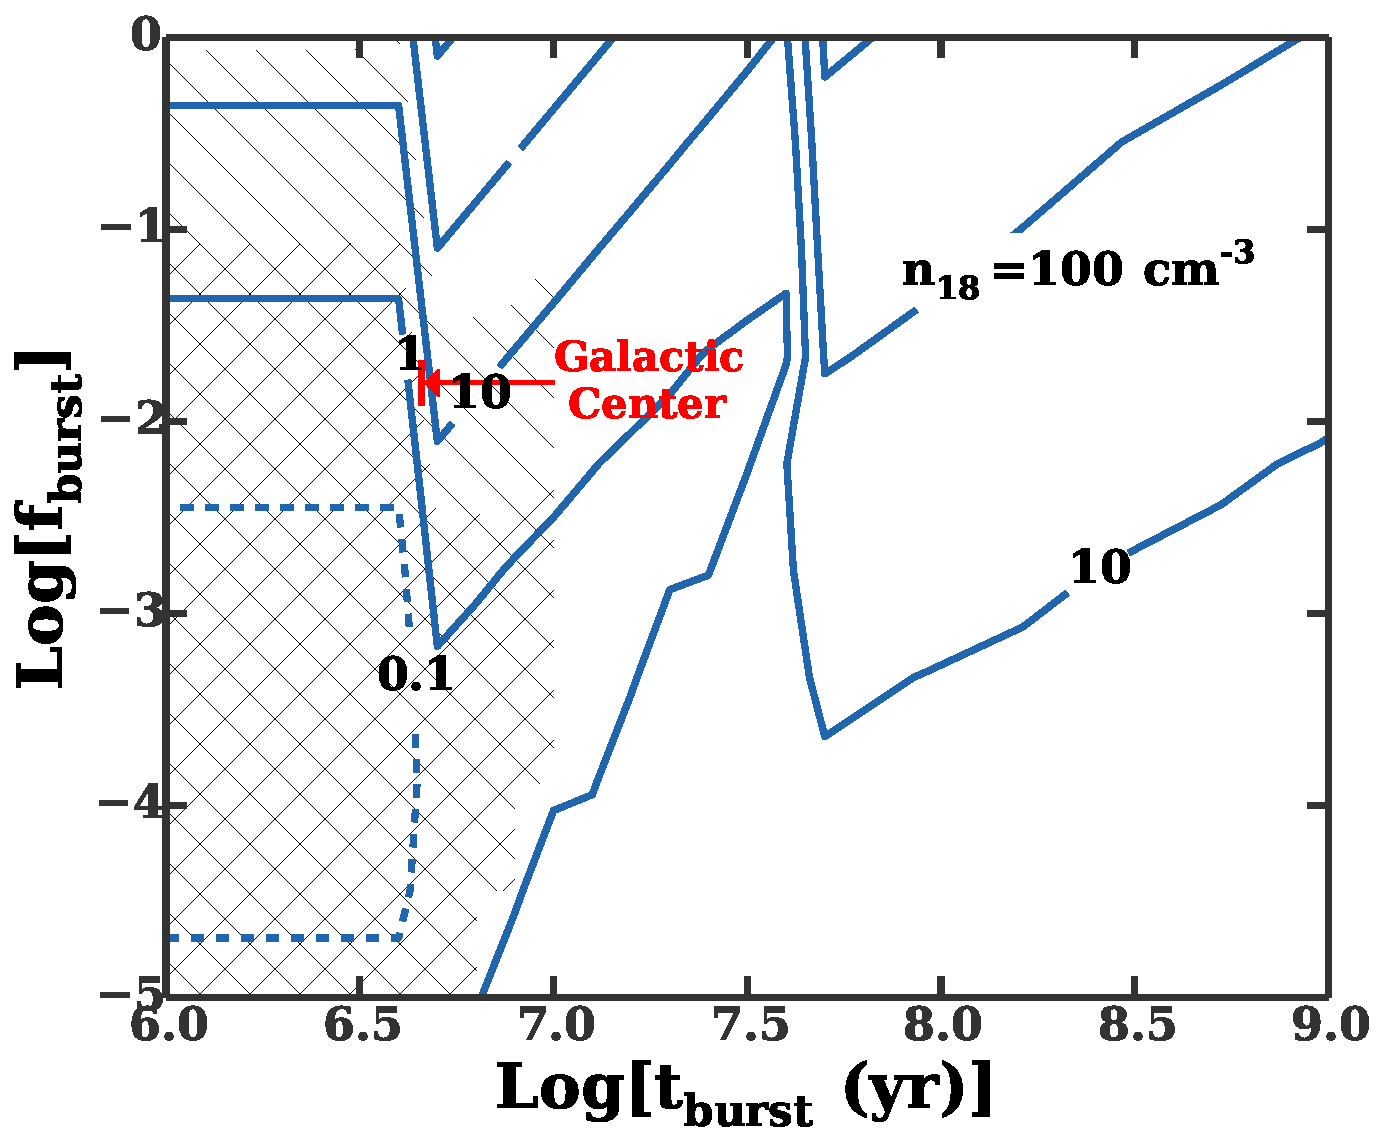
\includegraphics[width=8cm]{cnm_plot.pdf}
  \caption{\label{fig:param} Heating rates ($v_w$) and mass return
    parameters ($\eta$) for different star formation histories (gray
    lines). Solid, gray lines correspond to a star-burst of $<3$ Myr
    ago forming a fraction $f$ of the stars. The rest of the stars
    formed either a Hubble time ago (top line) or 1 Gyr ago (bottom
    line). The fraction $f$ increases and the gas density from left to
    right along these lines. The dashed, gray line corresponds to an
    alternate scenario in which there are two recent bursts in rapid
    succession in rapid succession: the older burst is $\sim 3$ Myr
    old (just at the point when stars are beginning to leave the main
    sequence). The contribution of this older burst increases towards
    the right, crossing boundary of the thermally unstable (``TI'')
    region below the thick black line. Iso-contours for the density at
    $10^{18}$ cm ($\mathrm{n_{18}}$) are shown as solid blue lines.} 
\end{figure}


\subsection{Alternative constraints on CNM gas density}
In this section we present alternative constraints on the CNM gas
density.  

We can translate observed distributions of Eddington ratio into 
distributions of $n_{18}$ using

\begin{equation}
m \dot{M}_{\rm Edd}= f_{\rm in} 4 \pi r^2 \mu m_p n v,
\label{eq:mdot}
\end{equation}

where $n$ is the average density at radius $r$ and $f_{\rm in}$
represents the fraction of the large scale inflow, which actually
accretes onto the black hole.  Using the free-fall velocity for
$v$, we obtain

\begin{equation}
n_{18} = 3 \times 10^6 M_7^{1/2} m \left(\frac{f_{\rm in}}{0.01}\right)^{-1} {\rm
  cm}^{-3}
\label{eq:n18Edd}
\end{equation}

\citet{Kauffmann+2009} present distributions of ${\rm L[OIII]}/\Mbh$,
for different bins of black hole mass (see their Figure 4).  Assuming
a bolometric correction, these can be translated into distributions of
Eddington ratio $m$.  According to \citet{Kauffmann+2009} ${\rm
  L[0III]}/\Mbh=1.7$, roughly corresponds to Eddington ratio of 1. We
adopt this conversion and assume that the bolometric correction is
independent of ${\rm L[0III]}/\Mbh$.

We focus on the distribution of Eddington ratios for low mass lack
hole bin ($10^7$ and $10^{7.25} \Msun$) in \citet{Kauffmann+2009}
(this is the cyan curve in left hand panel their Figure 4). The
distribution is well fit by

\begin{align}
  &F_{\rm cum}(m)=\frac{F_{m_0}}{2^{-1/s}}
  \left(\left(\frac{m}{m_0}\right)^{-a1\,
      s}+\left(\frac{m}{m_0}\right)^{-a2 \, s}\right)^{-1/s} \label{eq:khFit}\\
  &s, a1, a2, F_{m_0}=1.42, -0.166, -1.20, 0.235.\nonumber
\end{align}

We can use equation~\eqref{eq:n18Edd} to translate this into a cumulative
distribution of $n_{18}$. We show the corresponding distribution in
$n_{18}$ in Fig.~\ref{fig:n18Cum}.

\begin{figure}
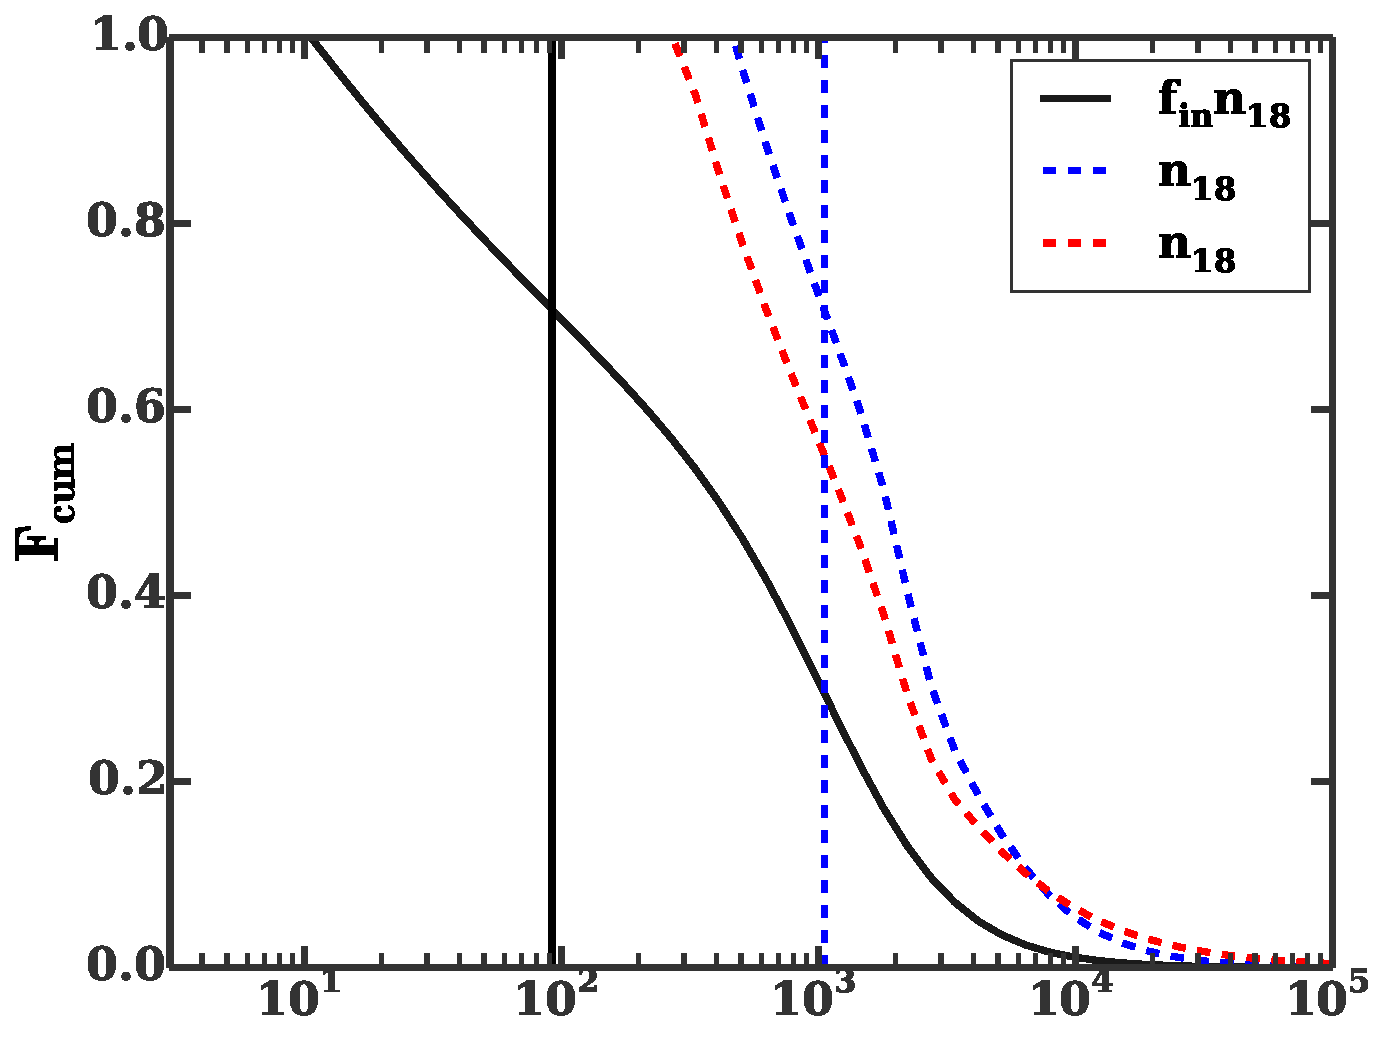
\includegraphics[width=8cm]{fcum_n18.pdf}
\caption{\label{fig:n18Cum} Fraction of black holes with $f_{\rm in}
  n_{18}$ greater than a given value--from equations~\eqref{eq:n18Edd}
  and~\eqref{eq:khFit}. Recall that $f_{\rm in}$ is the ratio of the
  true accretion rate onto the black hole to the inflow rate of
  free-falling gas at $10^{18}$ cm. 
% We expect $f_{\rm in}\approx
%   {10^{-3}-10^{-2}}$ for low densities and $f_{\rm in} n_{18} \simeq
%   1$ to be of order unity for $f_{\rm in} n_{18} \gsim 100 $.  In terms of
%   Eddington ratio, $m$, this corresponds to only a small fraction of
%   the large scale inflow reaching the hole for $m\lsim 0.01$, and an
%   order unity fraction reaching the hole for $m\gsim 0.01$.
}
\end{figure}

No galaxies have a $f_{\rm in }n_{18} \lsim$ few cm$^{-3}$.  This
gives a lower bound on $n_{18} \gsim$ few cm${-3}$.  This lower bound
would increase as $f_{\rm in}^{-1}$. However, measurements of
Eddington ratio below $\sim 10^{-3}$ are unreliable, so a small
fraction of galaxies ($\sim 20\%$), could have much lower gas
densities.

We expect that $f_{\rm in}$ could be quite small for highly sub
Eddington systems. For example, Faraday rotation measurements
\citep{Quataert+2000} show $f_{\rm in}\approx 10^{-3}$, in our own
galactic center. However, we expect $f_{\rm in}$ will be of order
unity for systems with $m\gsim 0.1$.  

In order to obtain the cumulative distribution for $n_{18}$, we need
a prescription for $f_{\rm in}$. We refer to \citet{Li+2013}, who
performed two-dimensional hydrodynamical simulations of axi-symmetric
rotating accretion flows. When the inflow rate on large scales was
very sub-Eddington ($\dot{M}/\dot{M}_{\rm Edd} \lsim 10^{-4}$),
cooling was inefficient and $f_{\rm in}$ was $\sim 0.01$. On the other
hand, when $\dot{M}/\dot{M}_{\rm Edd}\gsim 10^{-2}$, $f_{\rm in}$
approaches unity.  We use $\dot{M}_{\rm Acc}/\dot{M}_{\rm Bondi}$ in
their Figure 6 for $f_{\rm in}$.  With this choice only a third of
nuclei have $n_{18}>2,000$ and only 6\% have $n_{18}>10^{4}$ {\bf
  AG--TDEs could be subset which have very high or very low densities.}

Note that \citet{Li+2013} use an alpha viscosity prescription with
$\alpha=0.01$. We would expect that the value of $f_{\rm in}$ would be
sensitive to this choice. {\bf AG--a little more discussion of limitations.}

Two potential complications to keep in mind are (i) clumpiness of the
CNM and (ii) anistropy. The distributions above are
distributions of the {\it average} $n_{18}$.  Most likely, some of the
nuclear gas in a low density hot phase, while the rest is in high density
cold clumps/filaments. However, in this case the cold filaments would
be dissolved by the radiation from the jet...{\bf AG this needs
  justification/validation. If this is really true, then analytic
  section is faulty because it focuses on the hot phase.}

% {\bf AG Jeans criterion -- but be careful of tidal effects.}

AGN feedback would may blow low density bubbles in the
CNM. \citet{Russell+2013} used Chandra x-ray observations to measure gas
density and temperature profiles for a sample of massive elliptical
galaxies. The measured electron density on scales of $\sim 100
pc$ is $\gsim 0.1$ cm$^{-3}$. Note that the gas density at 100 pc
would be irrelevant for a TDE jet, but we would not expect the gas
density to be decreasing towards the galactic center in a steady
state. {\bf These are only massive ellipticals with $\Mbh\sim 10^{9} \Msun$.}

\subsection{Adopted gas density profiles}
 The following density provided a good fit to the CNM density profile
 of cusp galaxies.

\begin{align}
n=
\begin{cases}
  n_{18} \left(\frac{r}{10^{18} {\rm cm}}\right)^{-1} {\rm cm^{-3}} & r<r_b \\
  n(r_b) \left(\frac{r}{r_b}\right)^{-\beta} {\rm cm^{-3}} & r\geq
  r_b,\\
  \label{eq:profile}
\end{cases}
\end{align}

where $0.1 \Mbh[7]^{1/2} \lsim n_{\rm 18}\lsim 2,700
\Mbh[7]^{0.38} $ cm$^{-3}$.  

The gas density density experiences a break at radius $r_b$, the break
radius in the stellar density profile, where the stellar density
transitions from an inner power law slope $\delta_1\lsim 2$ to an outer
power law slope $\delta_2\gsim 2$. $r_b\gsim 100$ pc for cusp galaxies,
in which case the break radius may be safely ignored as it will be
well outside the jet deceleration radius. If there is a nuclear
star cluster present the effect $r_b$, the outer boundary of the
nuclear star cluster will correspond to a much smaller effective
$r_b\sim 1-5$ pc. However, even in this case the break radius is still
one too large scales to affect the light-curve evolution {\bf AG why?}
Thus, we don't include a break radius in our gas density profiles.

We perform simulations with CNM density $n=n_{18} \left(r/10^{18} {\rm
  cm}\right)^{-1}$ with $n_{18}$=2, 60, and 2000 to see what effect
varying the CNM density would have on the observed radio light-curve.

% The outer power law slope of the gas density will depend on the slope
% of the $\beta$ but will typically vary between 1.5 and 2. 

% We explore the parameter space of $n_{18}$, $\beta$, and $r_b$,
% adopting values for these parameters summarized by
% Table~\ref{tab:params} below


% \begin{table}
%   \caption{\label{tab:params} Summary of numerical parameters used for
%     the CNM profile (equation~\eqref{eq:profile}). A ``-'' in the $r_b$
%     or $\beta$ columns indicates that the gas density profile is a
%     single power law without any breaks. ``...'' in any column
%     indicates the entry is the same as the one above it.}
% \begin{minipage}{\columnwidth}
% \begin{tabular}{|l|l|l|}
% $n_{18}$ & $r_b [{\rm pc}]$ & $\beta$\\
% \hline
%   2     &  -    &  -\\
%   60    &  -    &  -\\
%   ...   &  1    &  1.5\\
%   ...   &  ...   &  2\\
%   2000  &  -    &  -\\
% \end{tabular}
% \end{minipage}
% \end{table}


{\bf AG cores...}

We also use a core galaxy profile to see how the shape of the stellar
density profile would affect the radio lightcurve. For core galaxies
the stellar density profile is not a pure power law. To simplify
things we will consider one particular slope for the stellar density
profile: $\rho_\star\sim r^{-\delta_1}$ with $\delta_1=1.1$. The gas
density profile may be approximated as

\begin{align}
\begin{cases}
n=n(r_s) k(x) & 0.4 \leq x\leq 2.0\\
n = 2.0 n(r_s) (x/0.4)^{-0.95} & x < 0.4\\
n = 0.75 n(r_s) (x/2.0)^{-0.26} & 2.0< x \leq r_s/r_b\\
n \sim x^{-1.5} & x>r_s/r_b\\
\end{cases}
\label{eq:cores}
\end{align}

Where, 

\begin{align}
  &x=r/r_s\\\nonumber
  &k(x)=\frac{45}{19} \frac{1}{x^{3/2}} \frac{1-x^{1.9}}{9-19
      x\frac{x^{0.9}-1}{x^{1.9}-1}}
\end{align}

To isolate the effects of the shape of the density profile, consider a
core density profile with $r_s=10^{18}$ cm, and $n_{18}=2000$: the
same as our high density cusp model.

% We consider a high density model (near the verge of thermal
% instability) and a low density model (near the lower limit of what
% stellar winds can give for the CNM density). The values $n(r_s)$ and
% $r_s$ are given in the table below. 

% \begin{table}
% \begin{tabular}{|l|l|l}
%  core models & $n(r_s)$ & $r_s$\\
% \hline
%  High & 2,500 $\Mbh[7]^{-0.32}$ cm$^{-3}$ &  4 $\times 10^{17}  
%  \Mbh[7]^{0.8}$ cm\\
%  Low & 0.1 $\Mbh[7]^{-0.24}$ cm$^{-3}$ & 6$\times 10^{16} \Mbh[7]$ cm
% \end{tabular}
% \end{table}

\section{TDE jets}
\label{sec:jet}
This section would summarize modeling of TDE jets.

\subsection{Jet Models}

\subsection{Hydrodynamics}

\subsection{1-d vs. 2-d Models}
\label{sec:2d}
We compare the light-curves for 1-d and 2-d jet simulations with the
same structure (fast ($\Gamma=10$) core and slow ($\Gamma=2$)
sheath). Note that the hydrodynamic evolution of these 2 components is
independent in 1-d, but the radiative transfer/light-curve calculation
is sensitive to the jet geometry.

For the both the 1-d and 2-d simulations, we take a half opening angle
of $\theta=$0.1 radians for the fast ($\Gamma=10$) core of the
jet. For the 2-d simulations, we assume the slow component initially
spreads from $\theta=$0.1-0.5 radians. This component quickly spreads
out in a high density medium ($n_{18}=2000$), becoming
quasi-spherical. Thus, the slow component to a good approximation
covers all solid angles not covered by the fast component. We set the
isotropic equivalent energy in the 1-d simulations accordingly...

We show a comparison of this modified 1-d approach with the true
2-d result in Figure~\ref{fig:1d2dB}, for $n_{18}=60$ and
$n_{18}=2000$...

\begin{figure*}
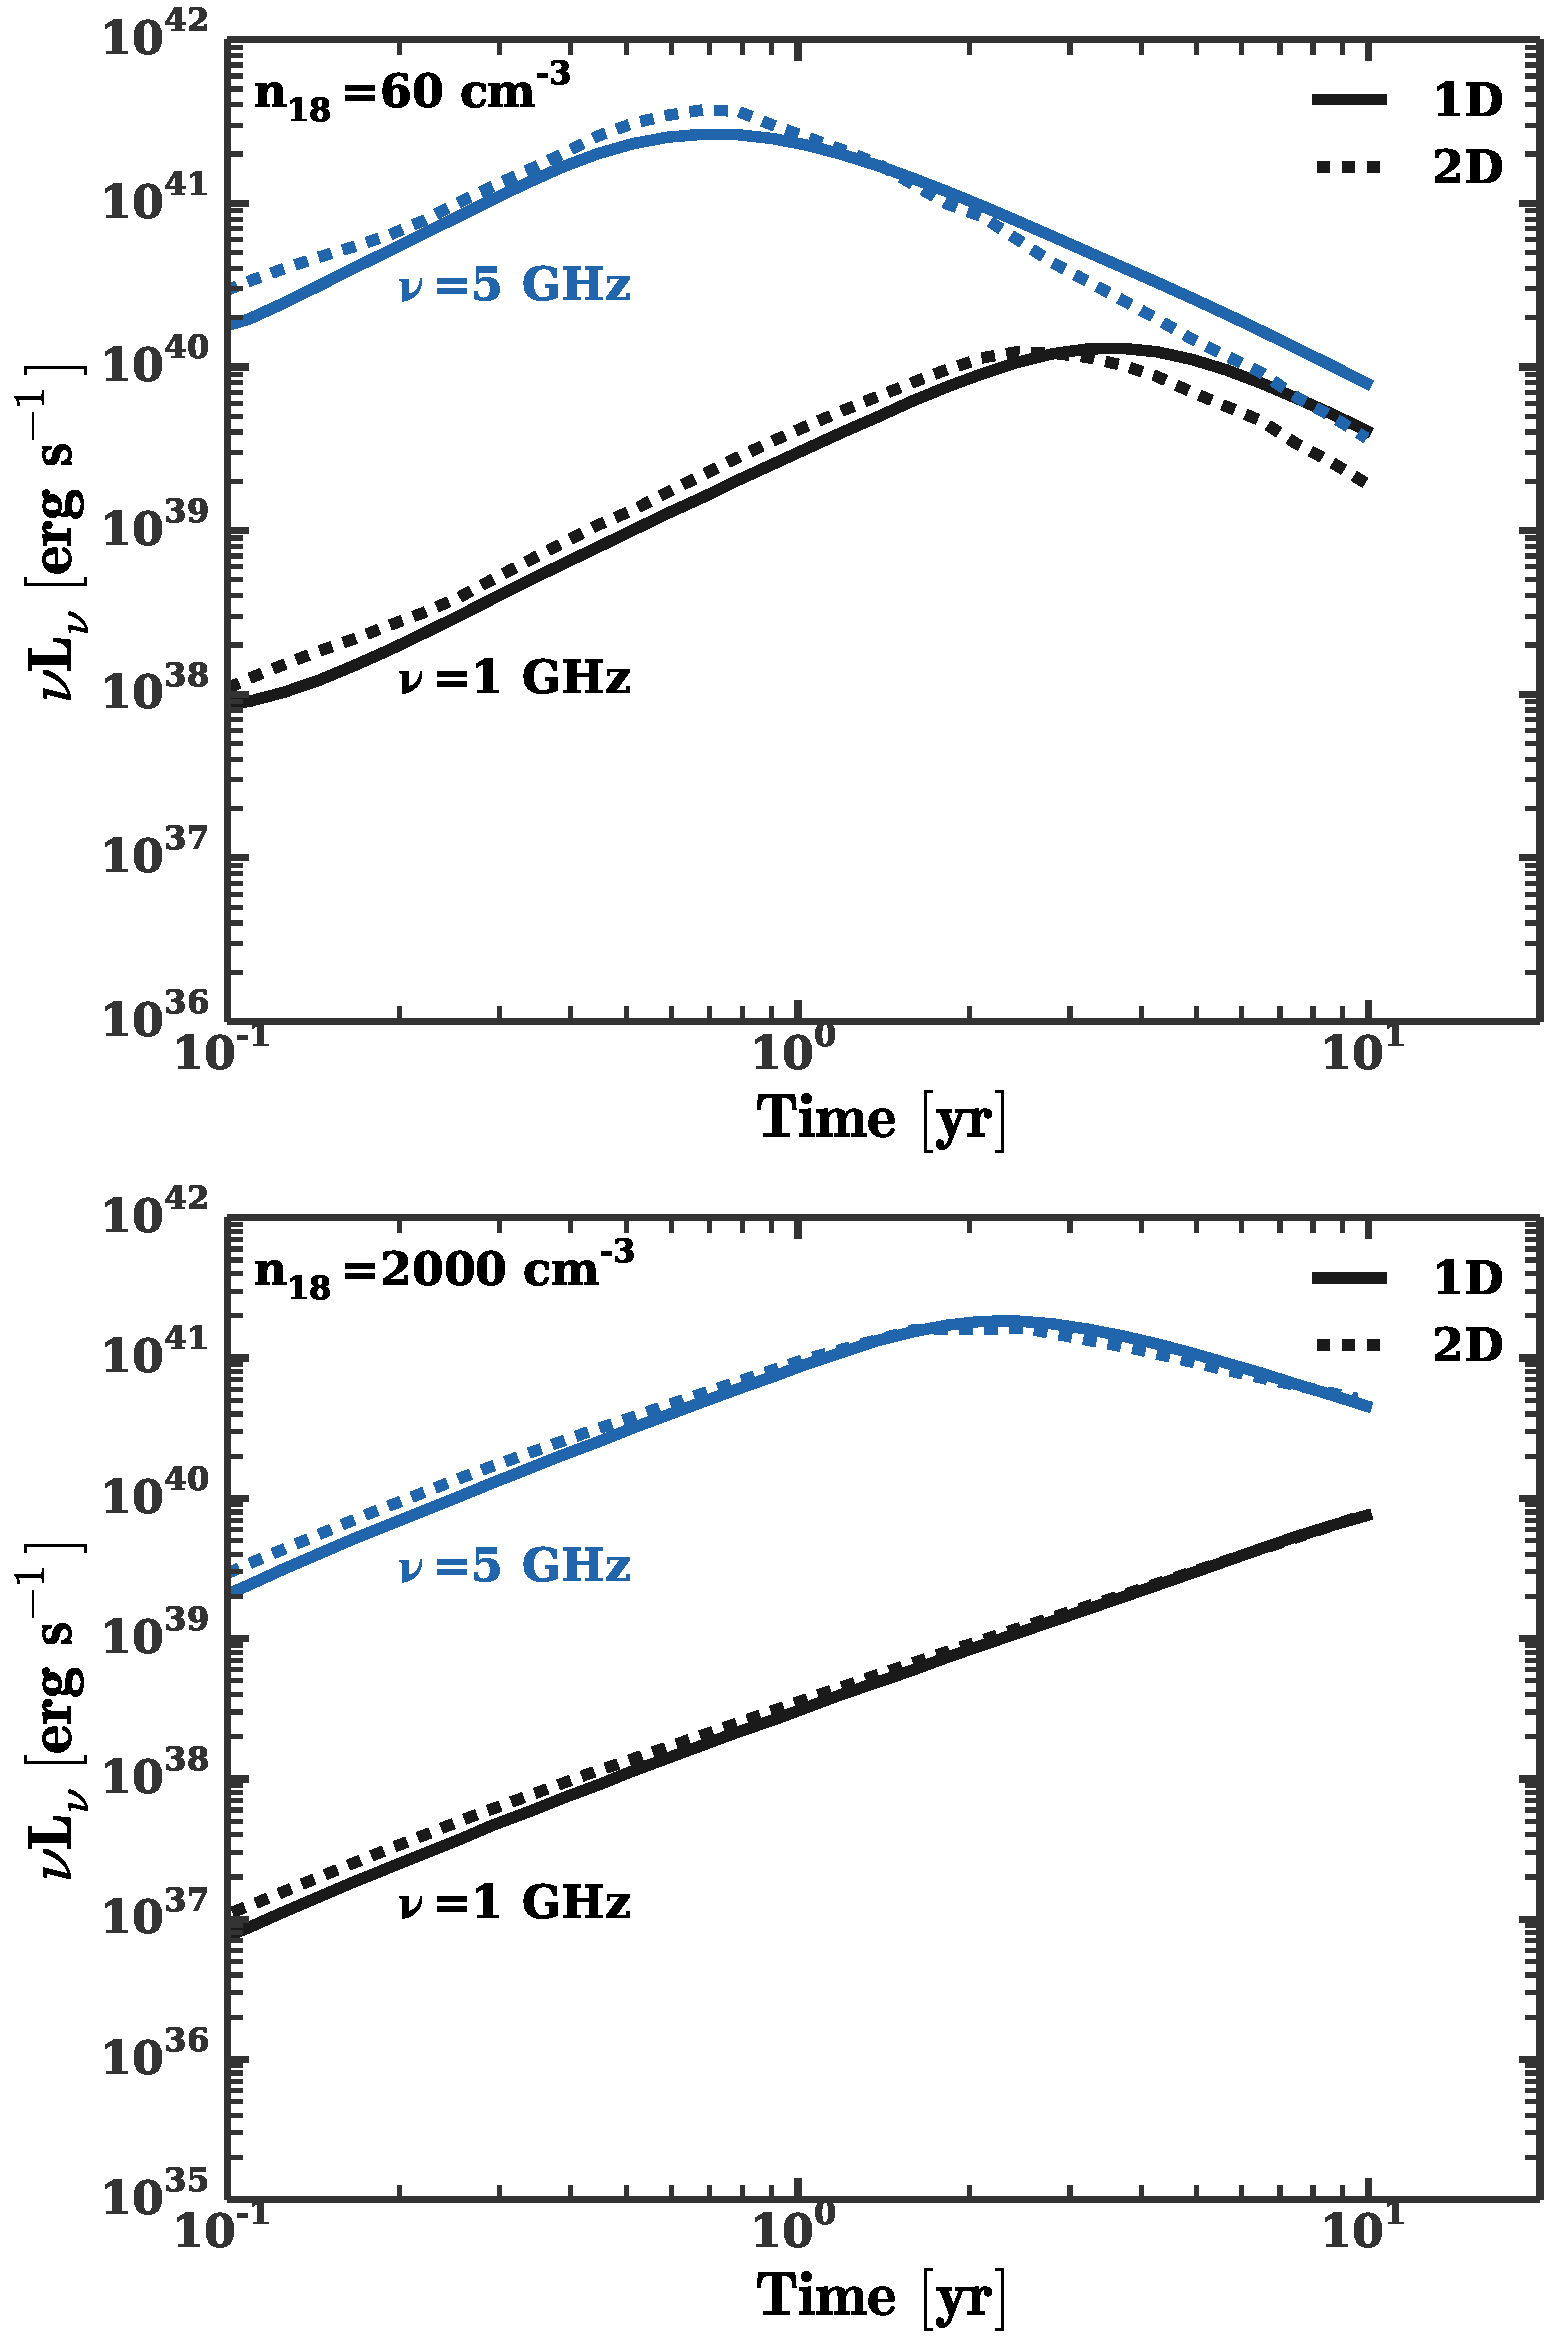
\includegraphics[width=16cm]{1d_2d.pdf}
\caption{\label{fig:1d2dB} Comparison light-curves for $n_{18}=60$
  (top) and $n_{18}=2000$ (bottom) for frequencies of 1 GHz (left) and
  30 GHz (right) and an observer angle of 0.8 radians to the jet
  axis. We assume an $n\sim r^{-1}$ density profile for $n_{18}=2000$,
  but take $n\sim r^{-1.5}$ for $n_{18}=60$ for computational
  convenience.}
\end{figure*}


\section{Results}
\label{sec:results}

\subsection{Effects of gas density}

In Fig.~\ref{fig:upper_limits} we show the on-axis light curves for
our fiducial jet model and CNM density profile $n=n_{18} (r/10^{18}
{\rm} cm)^{-1}$ cm$^{-3}$ with $n_{18}$=2, 60, and 2000 cm$^{-3}$. The
higher density models peak at later times with smaller peak
luminosities {\bf AG Do we understand this? Is this due to the effect
  of self-absorption?}

{\bf AG it would probably be good to have a figure showing the
  different components contributing to the emission.} The radio light
curve has contributions from both the slow and fast jet
components. The fast component dominates at
early times for the $n_{18}=2$ and 60 lightcurves, while the slow
component dominates for all times as frequencies for
$n_{18}$=2000. Generally, the fast component is more important at
higher frequencies, and lower densities.

We also show radio upper limits and detections for various TDE
candidates in Fig.~\ref{fig:upper_limits} (these were compiled from
various sources into Table 1 of \citealt{Mimica+2015}). Overall, the
measurements were taken too late to be strongly constraining,
especially for the low density models: the lightcurves or $n_{18}=2$
peak on time-scales of months, while many of the radio measurements
were taken decades after the TDE flare.

\begin{figure} 
  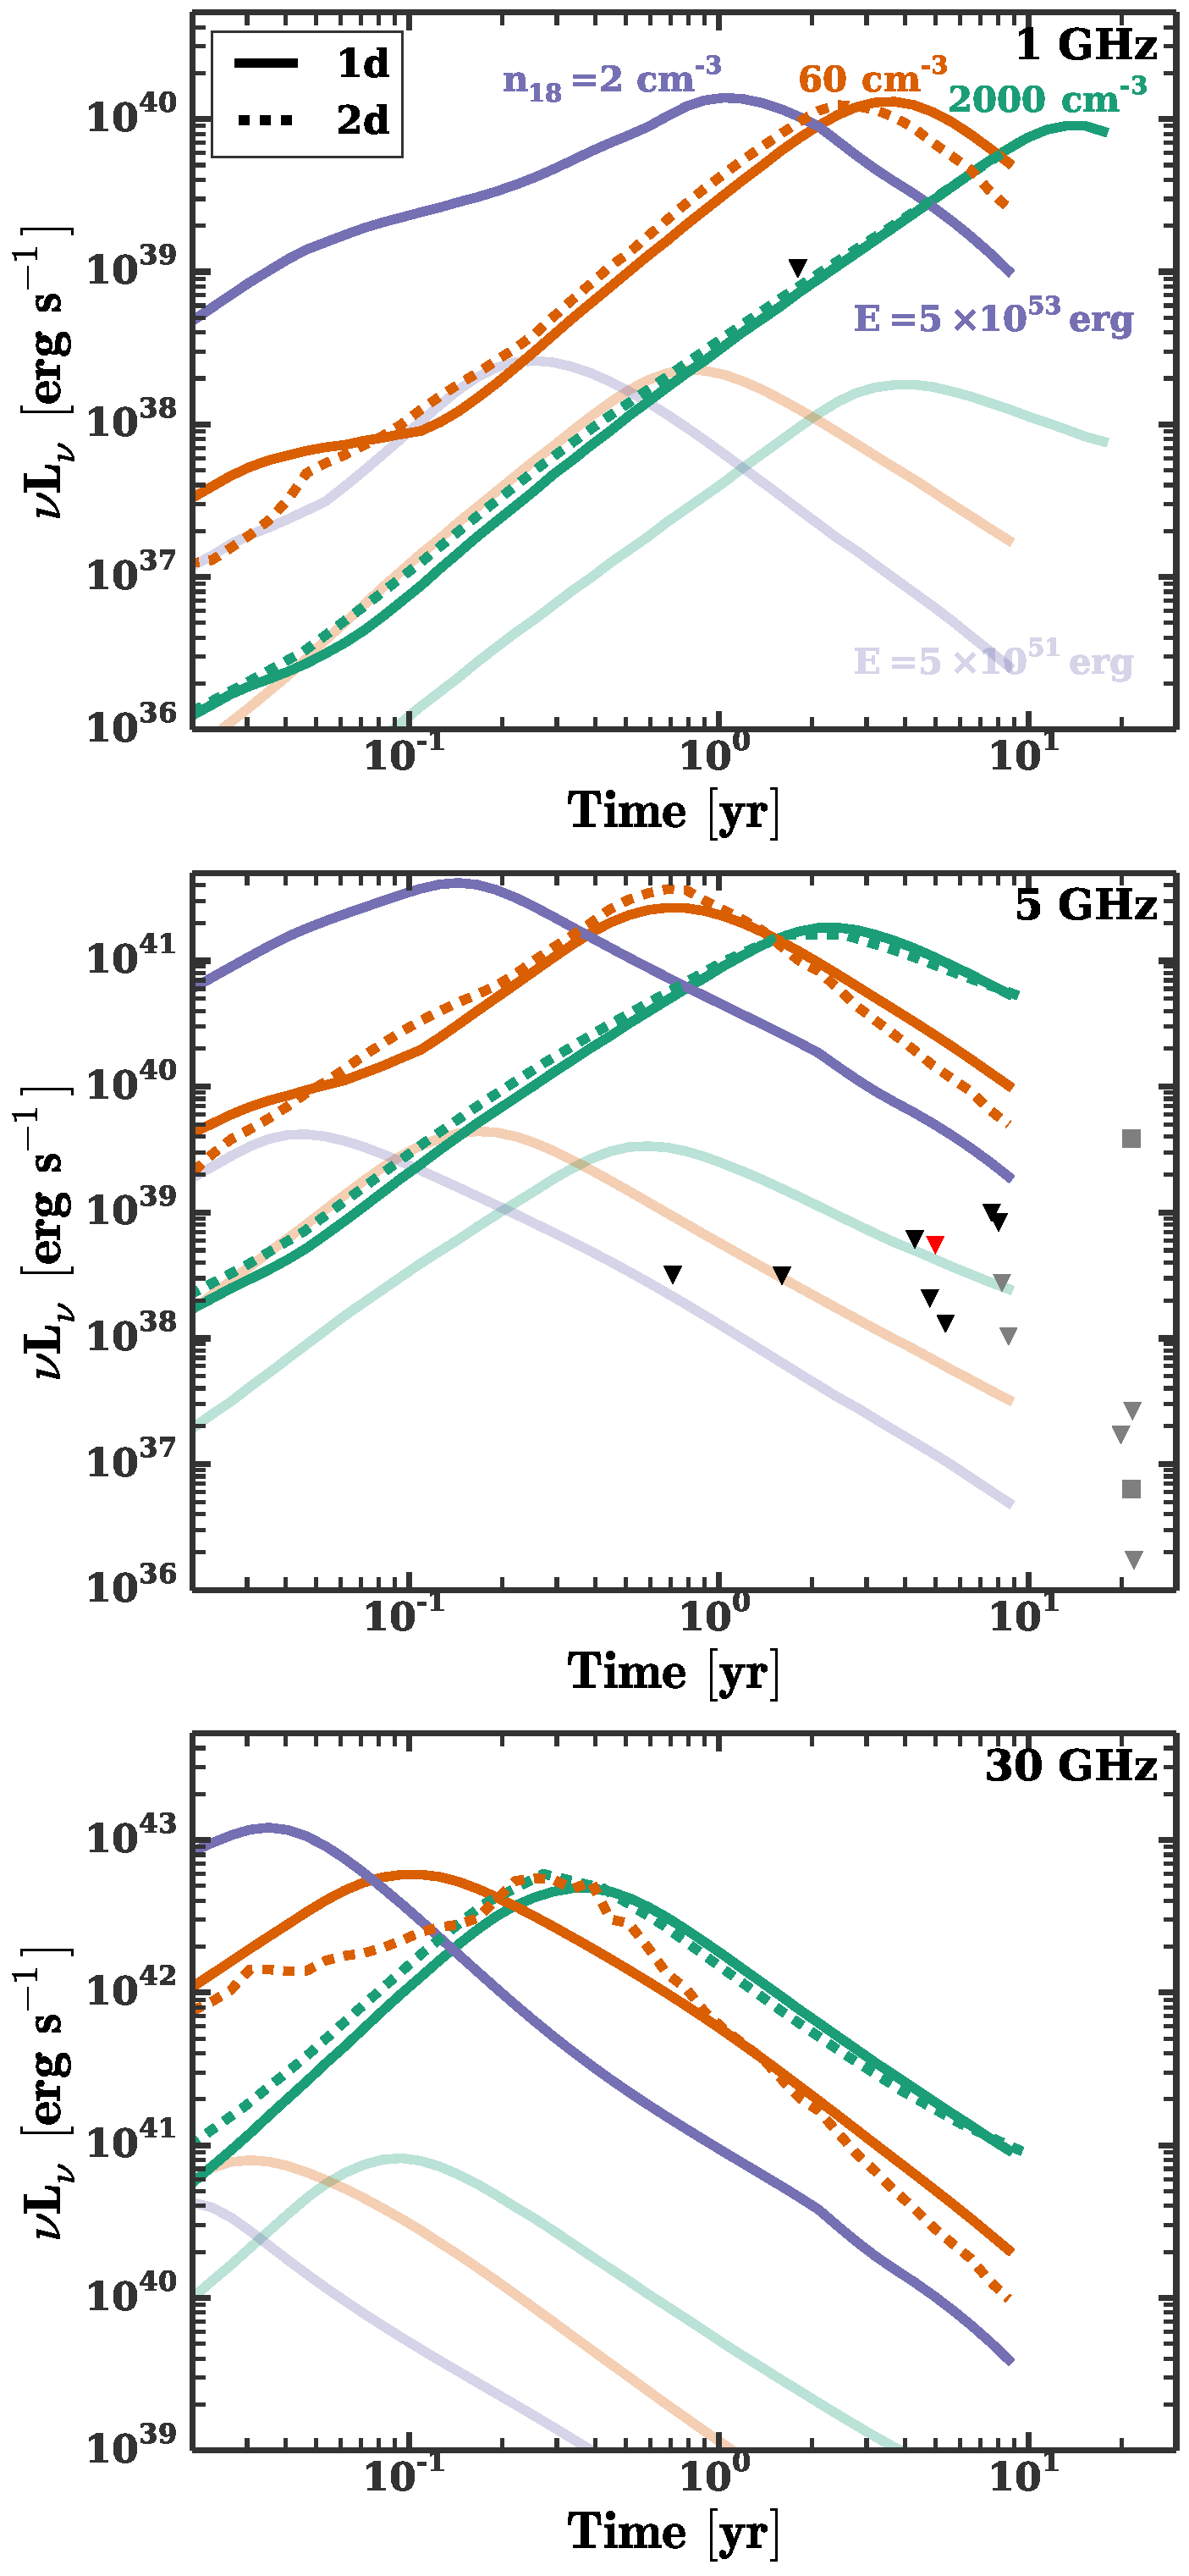
\includegraphics[width=8cm]{lightcurves.pdf}
  \caption{\label{fig:upper_limits} On-axis radio light-curves for
    fiducial jet model and CNM density profile $n=n_{18} (r/10^{18}
    {\rm cm})^{-1}$, for three different values of n$_{18}$: 2, 60,
    and 2000. Radio upper limits and detections are shown as
    black/gray triangles and squares respectively (compiled in Table 1
    of \citealt{Mimica+2015}). The single upper limit in the top panel
    corresponds to 1.4 GHz. Gray triangles and squares in the middle
    panel indicate upper limits and detections at 3.0 GHz, while black
    triangles indicate upper limits at 5.0 GHz.}
\end{figure}

\subsection{Effect of gas density profile}
We have also computed the radio light-curves for different shapes of
the gas density profile, while holding $n_{18}$ fixed. We compute the
results for $n_{18}=2000$ for both our fiducial $n\sim r^{-1}$ profile and
the core galaxy profile, shown in equation~\eqref{eq:cores}. The
former would more relevant for a cuspy stellar density profile with
stellar density $\rho_{\star}\sim r^{-2}$, while the latter would be more
appropriate for a flatter $\rho_{\star}\sim r^{-1}$ stellar density
profile. As a steeper stellar density is more favorable for producing
tidal disruption events, we would expect most events to occur is cusp
rather than core galaxies.

The results are virtually indistinguishable as shown in
Fig.~\ref{fig:cores}. Overall, the late time evolution of the
light-curve is insensitive to the slope of the stellar density profile
(see Figure 3 of \citealt{Mimica+2015}) {\bf AG this is only for the
  fast narrow component--how do we justify this more generally?}.


\begin{figure} 
  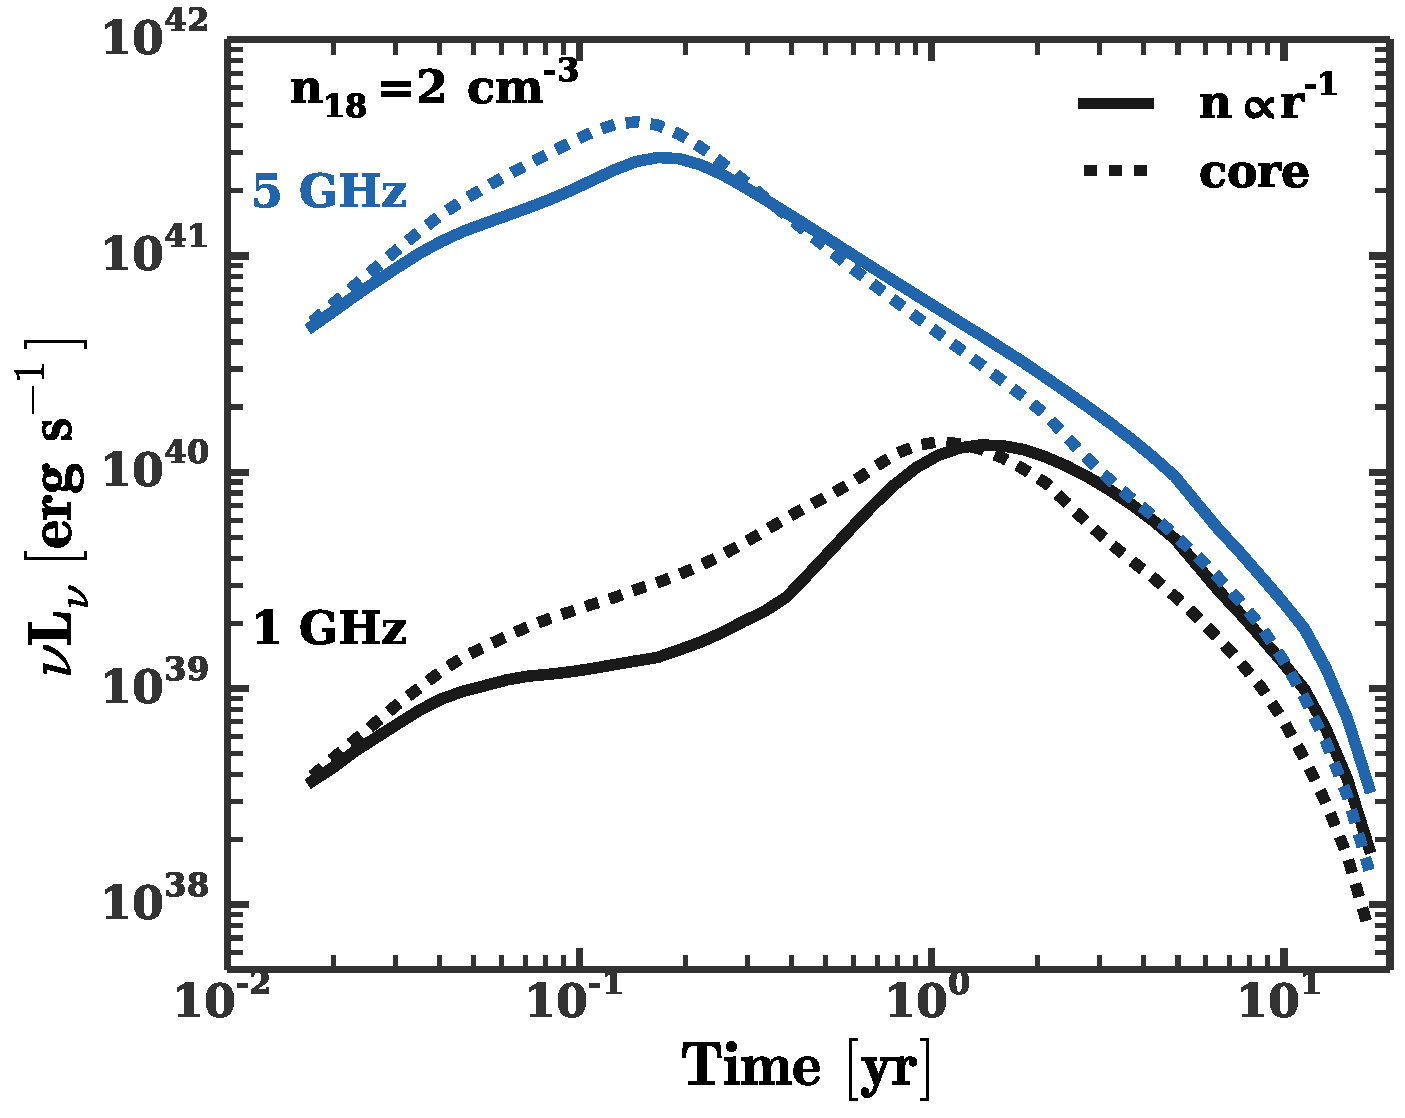
\includegraphics[width=8cm]{fig_cores.pdf}
  \caption{\label{fig:cores} Comparison of the light-curves for
    $n_{18}=2000$ and two different CNM gas density profiles: $n\sim
    r^{-1}$ and the core galaxy profile from \eqref{eq:cores} with
    $r_s=10^{18}$ cm and $n(r_s)=2000$, so that we can isolate the
    effect of the shape of the density profile. 4 pi correction}
\end{figure}


\subsection{Effects of viewing angle}


\section{Discussion}
\label{sec:disc}
{\bf AG -- Observational prescriptions and rates?}

\section{Summary and Conclusions}
\label{sec:conc}

\clearpage
  \footnotesize{
    \bibliographystyle{mnras}
    \bibliography{master}
  }

\end{document}
